\section{Experiments}
\label{sec:experiments}
\paragraph{Study design.}
We compare AdamW, SGD with momentum (SGD-M), balance-only, and
QuotientOpt. Balance-only uses the same section change, transported
first moment, and factor step as QuotientOpt, omitting the Sylvester
projection. Geometric runs use normalized EMA momentum,
$\beta=0.9$, regularization $\varepsilon=10^{-6}$, and balance interval
one; SGD-M uses its library momentum convention. Equal tuning budgets
apply to all four methods. Shared non-factor optimization and all data
protocols are specified in Appendix~\ref{app:full-protocol}.

The additional four-task search contains 208 attempts: 13 optimizer
settings per method and task, with 1000 epochs for graphs and 2000 for
regression. Of these, 186 complete the full horizon and 22 terminate
numerically. We then freeze parent-selected learning rates and complete
36 initialization checks, varying model initialization over 42, 43,
and 44 while holding data and shuffle seed 42 fixed. All 244 additional
attempts have therefore finished. Every stopped run and finite prefix
is recorded in Appendix~\ref{app:new-task-expansion}; the original
exhaustive proposal grid is tracked separately.

\begin{figure*}[t]
\centering
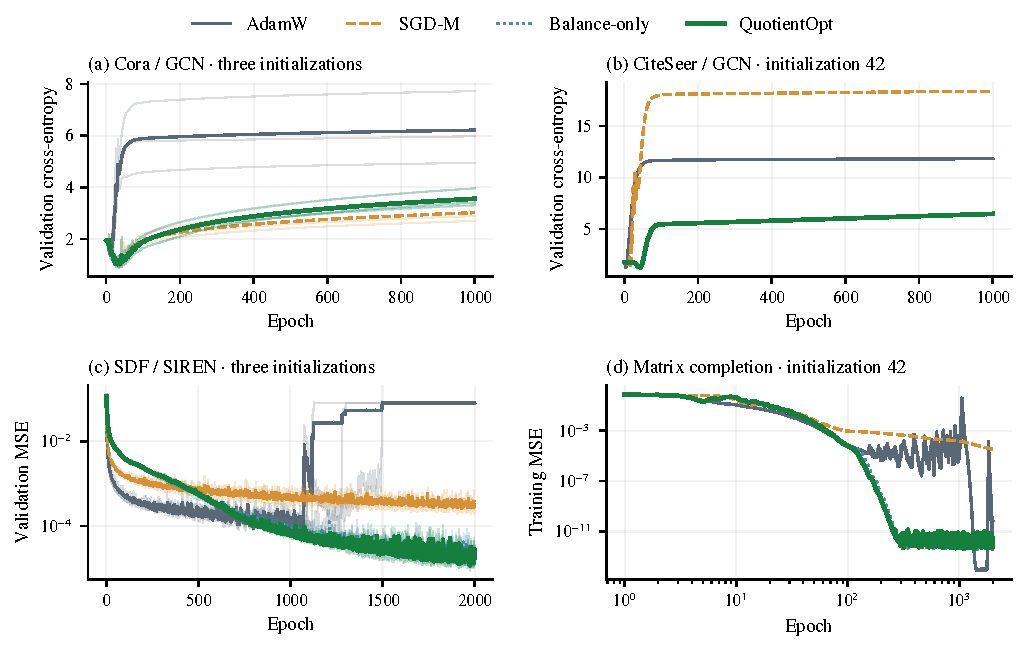
\includegraphics[width=.99\textwidth]{figures/icml_core_losses.pdf}
\caption{\textbf{Complete loss trajectories across three task families.}
All methods and recorded epochs are retained, without smoothing.
(a,c) Thin lines show three model initializations and thick lines their
arithmetic mean, using fixed data and frozen parent-selected learning
rates. (b) CiteSeer: actual minimum-validation-CE selected runs over
equal 13-setting budgets, seed 42. (d) Matrix completion: actual runs
selected by earliest validation hit of the $10^{-4}$ relative-MSE
target; SGD-M uses its minimum-validation-loss completed run because it
never hits this target. Both axes in (d) are logarithmic. Test outcomes
and iteration counts are in Table~\ref{tab:main-results}; complete
records appear in Appendices~\ref{app:new-task-expansion}--\ref{app:initialization-confirmation}.}
\label{fig:main-loss}
\end{figure*}

\paragraph{Selection protocol.}
The earliest minimum-validation-loss checkpoint selects the model;
the lowest validation loss selects the configuration, with deterministic
LR and epoch tie breaks. Test metrics enter neither decision.
Cora and CiteSeer use public transductive splits, a rank-4 GCN input
adapter, and cross-entropy (CE). The synthetic sphere SDF uses a rank-8
SIREN and MSE. Matrix completion uses a $128\times128$ planted rank-8
matrix of condition 100 with disjoint 50/10/40\% train/validation/test
masks. The original accuracy-selected Cora analysis and all seven
learning rates are retained in Appendix~\ref{app:fresh-evidence-cases}.

\paragraph{Graph prediction and implicit representations.}
Across three fixed-data model initializations, QuotientOpt reduces
Cora test CE from AdamW's $1.1376$ to $0.8807$, a $22.6\%$ mean
reduction, with lower loss in all three pairs. SGD-M achieves $0.8741$
and balance-only $0.8807$. On CiteSeer at seed 42, QuotientOpt gives
test CE $1.2163$, versus $1.3762$ for AdamW and $1.2508$ for SGD-M;
balance-only gives $1.2168$. The corresponding accuracies are
$65.1\%$, $45.7\%$, $54.2\%$, and $65.1\%$.

For SDF fitting, three-initialization mean test MSE is
$1.10\times10^{-5}$ for QuotientOpt, $6.21\times10^{-5}$ for AdamW,
$2.62\times10^{-4}$ for SGD-M, and $1.18\times10^{-5}$ for
balance-only: mean reductions of $82.2\%$, $95.8\%$, and $6.2\%$.
Paired lower-loss counts are $3/3$, $3/3$, and $2/3$.
The joint 13-setting seed-42 selection gives test MSE
$9.36\times10^{-6}$ versus AdamW's $6.03\times10^{-5}$; this comparison
also holds when finite checkpoints from subsequently stopped trials
are eligible. Table~\ref{tab:main-results} reports sample SDs conditional
on the fixed data split and frozen optimizer configurations.

\paragraph{Matrix-completion iteration counts.}
With a common initial validation scale and equal 13-setting budgets,
the seed-42 relative-MSE target $10^{-4}$ is first attained at epochs
107, 117, and 138 for QuotientOpt, balance-only, and AdamW; SGD-M does
not reach it by epoch 2000. This gives $22.5\%$ fewer validation-target
iterations than AdamW in the seed-42 tuning comparison.
Across the frozen-configuration initialization checks, target
attainment is $2/3$ for QuotientOpt and $3/3$ for AdamW;
Table~\ref{tab:matrix-initialization} gives every count. Final MSEs,
additional targets, Burgers/DeepONet outcomes, and all stopped runs
appear in Table~\ref{tab:new-task-scores} and
Appendix~\ref{app:new-task-expansion}.

\paragraph{Poisson/PINN fixed-setting result.}
In a completed four-method cohort of the original proposal grid,
the rank-16 Poisson/PINN configuration at learning rate $10^{-3}$
and seed 42 reaches 2000 epochs for every method. Its final held-out
relative $L_2$ errors are $0.05384$ for QuotientOpt, $0.05577$ for
balance-only, $0.06223$ for AdamW, and $0.07767$ for SGD-M.
Thus the QuotientOpt endpoint is $13.5\%$ below AdamW's and $3.5\%$
below balance-only's at this one matched setting. This is a
fixed-configuration comparison, not a completed full-grid selection;
all 26 complete four-method cohorts, including unfavorable ones, are
reported in Table~\ref{tab:new-results}.

\paragraph{Poisson/PINN across model initializations.}
Keeping the same data, shuffle, and rank-16 optimizer settings, we
freeze the original learning rate $10^{-3}$ and run model
initializations 43 and 44 for all four methods. Together with the
pre-existing initialization 42, each method has three completed
2000-epoch runs. Selecting checkpoints only by validation MSE, the
mean held-out relative $L_2$ error is $0.04971\pm0.00297$ for
QuotientOpt, $0.06163\pm0.00299$ for AdamW,
$0.07221\pm0.00698$ for SGD-M, and $0.04977\pm0.00302$ for
balance-only, where the dispersion is sample SD. QuotientOpt reduces
the mean by $19.4\%$ versus AdamW and $31.2\%$ versus SGD-M, with
lower test error in all three paired initializations against each.
Against balance-only, the mean difference is $0.13\%$ and the paired
count is $1/3$; these outcomes do not isolate an accuracy gain from
horizontal projection. Table~\ref{tab:poisson-initializations} and
Figure~\ref{fig:poisson-initialization-loss} give the full paired
comparison, and Table~\ref{tab:poisson-initialization-all} retains
each selected and final-horizon endpoint.
\begin{table}[t]
\centering\small
\setlength{\tabcolsep}{3pt}
\caption{\textbf{Frozen Poisson/PINN initialization check.} Validation-MSE-selected held-out relative $L_2$ error, rank 16, 2000 epochs, learning rate $10^{-3}$. Data and shuffle seed are fixed at 42; columns vary only model initialization. Mean $\pm$ sample SD is conditional on that fixed data. All four methods use the same frozen settings.}
\label{tab:poisson-initializations}
\begin{tabular}{@{}lrrrr@{}}
\toprule
Method & 42 & 43 & 44 & Mean $\pm$ SD\\
\midrule
AdamW & 0.06143 & 0.05875 & 0.06472 & 0.06163 $\pm$ 0.00299\\
SGD-M & 0.07777 & 0.06438 & 0.07450 & 0.07221 $\pm$ 0.00698\\
Balance-only & 0.05022 & 0.04655 & 0.05255 & 0.04977 $\pm$ 0.00302\\
\rowcolor{oursbg}\textbf{QuotientOpt} & 0.04994 & 0.04663 & 0.05255 & \cellcolor{oursgoodbg}\textbf{\boldmath 0.04971 $\pm$ 0.00297}\\
\bottomrule
\end{tabular}
\end{table}

\begin{figure}[t]
\centering
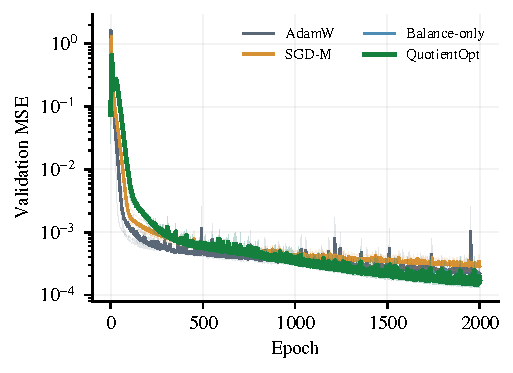
\includegraphics[width=.98\columnwidth]{figures/poisson_initialization_loss.pdf}
\caption{\textbf{Poisson/PINN validation loss.} Rank 16, fixed
learning rate $10^{-3}$, common data and shuffle seed 42. Thin lines
show every model initialization (42, 43, 44); thick lines are their
arithmetic mean at each epoch. All 2000 validation-MSE observations
per run are shown without smoothing. Held-out outcomes are in
Table~\ref{tab:poisson-initializations}.}
\label{fig:poisson-initialization-loss}
\end{figure}

\paragraph{Adjusted-run recovery.}
All 22 numerical stops in the additional task search were retried
from their original initial models with lower factor learning rates.
Each adjusted run reaches 2000 epochs. Within its separate retry
budget, validation MSE selects the configuration and checkpoint.
On Burgers/DeepONet, QuotientOpt's selected test MSE decreases from
$4.21\times10^{-3}$ in its original 13-setting search to
$2.47\times10^{-3}$ among seven adjusted runs, a $41.5\%$ reduction.
On SDF/SIREN, SGD-M's test MSE decreases from $2.42\times10^{-4}$
to $1.09\times10^{-4}$ among six adjusted runs, a $55.0\%$
reduction. The original matched-budget comparisons in
Table~\ref{tab:new-task-scores} remain the primary task results.
The other three retry groups complete the horizon with higher
validation-selected test MSE than their original group best:
SDF balance-only rises from $1.10\times10^{-5}$ to
$1.35\times10^{-4}$, SDF QuotientOpt from $9.36\times10^{-6}$ to
$1.40\times10^{-4}$, and matrix-completion SGD-M from
$1.17\times10^{-8}$ to $2.48\times10^{-8}$.
AdamW's original Burgers test MSE, $8.66\times10^{-5}$,
is still below the adjusted QuotientOpt result.
Table~\ref{tab:retry-summary} reports every retry group, and
Appendix~\ref{app:failure-retry} lists all 22 outcomes.
\begin{table*}[t]
\centering\small
\renewcommand{\arraystretch}{1.18}\setlength{\tabcolsep}{5pt}
\caption{\textbf{Adjusted fixed-step follow-up after numerical stops.} Every one of the 22 retried configurations reaches 2000 epochs from the bitwise-identical parent initial model. Only the factor learning rate changes. Within each task/method row, the retry setting and checkpoint minimize validation MSE. Original test MSE is the best of the preceding equal 13-setting search, also selected by validation MSE. Relative reduction is $100(1-\mathrm{retry}/\mathrm{original})\%$; a negative value means higher test MSE after retry. The retry counts are a separate tuning budget. Bold indicates a lower test MSE within the same method. All 22 outcomes are in Table~\ref{tab:retry-all}.}
\label{tab:retry-summary}
\begin{tabular}{@{}lrrrrr@{}}
\toprule
Task / method & Completed & Retry LR & Original test MSE $\downarrow$ & Retry test MSE $\downarrow$ & Relative reduction\\
\midrule
\rowcolor{oursbg}\textbf{Burgers / DeepONet / QuotientOpt} & 7/7 & 0.00255 & 0.0042 & \cellcolor{oursgoodbg}\textbf{\boldmath 0.0025} & +41.5\%\\
SDF / SIREN / SGD-M & 6/6 & 0.0085 & $2.42\!\times\!10^{-4}$ & \textbf{\boldmath $1.09\!\times\!10^{-4}$} & +55.0\%\\
SDF / SIREN / Balance-only & 3/3 & 0.85 & $1.10\!\times\!10^{-5}$ & $1.35\!\times\!10^{-4}$ & -1125.4\%\\
\rowcolor{oursbg}\textbf{SDF / SIREN / QuotientOpt} & 3/3 & 0.55 & $9.36\!\times\!10^{-6}$ & $1.40\!\times\!10^{-4}$ & -1391.8\%\\
Matrix completion / SGD-M & 3/3 & 0.255 & $1.17\!\times\!10^{-8}$ & $2.48\!\times\!10^{-8}$ & -111.6\%\\
\bottomrule
\end{tabular}
\end{table*}


\begin{table*}[t]
\centering\small
\renewcommand{\arraystretch}{1.18}\setlength{\tabcolsep}{5pt}
\caption{\textbf{Twelve-gauge sensing control.} Rank 4, 1000 updates, seed 42. $\Delta_T=\|X_T^{(Q)}-X_T^{(I)}\|_F/\|X_*\|_F$; the maximum uses completed gauges. $\bar\rho_{\rm upd}$ is mean update-direction vertical energy. Identity error reports final reconstruction without gauge perturbation. Failed gauges remain counted. All individual gauges and recovery controls are in Appendices~\ref{app:fresh-evidence-cases} and~\ref{app:failure-recovery}.}
\label{tab:main-gauge}
\begin{tabular}{@{}lrrrr@{}}
\toprule
Method & Finished & Max. $\Delta_T\downarrow$ & $\bar\rho_{\rm upd}\downarrow$ & Identity error $\downarrow$\\
\midrule
AdamW & 12/12 & $1.07\!\times\!10^{0}$ & $1.35\!\times\!10^{-1}$ & \textbf{\boldmath 0.0460}\\
SGD-M & 7/12 & $8.86\!\times\!10^{-1}$ & $5.65\!\times\!10^{-5}$ & 0.3797\\
Balance-only & 12/12 & $5.40\!\times\!10^{-5}$ & $1.91\!\times\!10^{-6}$ & 0.9994\\
\rowcolor{oursbg}\textbf{QuotientOpt} & 12/12 & \cellcolor{oursgoodbg}\textbf{\boldmath $5.20\!\times\!10^{-5}$} & \cellcolor{oursgoodbg}\textbf{\boldmath $1.20\!\times\!10^{-14}$} & 0.9994\\
\bottomrule
\end{tabular}
\end{table*}

\paragraph{Gauge robustness and horizontal state.}
Twelve scalar or dense gauges act on the same initial product, with
1000 updates per attempt. Table~\ref{tab:main-gauge} separately reports
product disagreement, update-direction vertical energy, and
identity-gauge reconstruction error. QuotientOpt has maximum completed
final disagreement $5.20\times10^{-5}$ and mean vertical energy
$1.20\times10^{-14}$; balance-only gives $5.40\times10^{-5}$ and
$1.91\times10^{-6}$. AdamW has smaller identity-gauge reconstruction
error and maximum gauge disagreement $1.07$. These measurements connect
horizontal memory to representation consistency while distinguishing
it from objective minimization. Complete sensing-loss histories appear
in Figure~\ref{fig:core-gauge-loss}; all gauges and replay controls are
retained in Appendices~\ref{app:fresh-evidence-cases}
and~\ref{app:failure-recovery}.

\paragraph{RU01 proposal-grid audit and focused continuation.}
At the November 4, 2026, 13:05 EST scope decision, 158 formal runs had
completed their prescribed horizons, including 115 main configurations;
26 task/rank/setting cohorts had all four methods. Five fixed-step gauge
runs retained failure status, and four active runs were paused with
checkpoints preserved. The nineteen completions since the earlier
139-run snapshot span all seven task families.
At one newly paired Cora/GCN hidden-adapter setting ($r=4$,
learning rate $10^{-3}$), the final test accuracies are $77.7\%$ for
QuotientOpt and $77.1\%$ for AdamW. SGD-M and balance-only were still
pending for that setting. In the newly complete CIFAR-10/MLP rank-32
cohort, QuotientOpt reaches $47.24\%$ final test accuracy versus
$49.42\%$ for AdamW, $47.82\%$ for SGD-M, and $47.23\%$ for
balance-only. These are fixed-setting final endpoints, not winners
from the full validation-selected search. In rank-16 matrix sensing,
the complete cohort has final reconstruction errors $0.92767$ for
QuotientOpt and $0.02616$ for AdamW. All nineteen new records,
including unfavorable results, appear in Table~\ref{tab:ru01-latest};
all complete four-method cohorts remain in Table~\ref{tab:new-results}.
The remaining exhaustive queue is replaced by a frozen-configuration
Poisson/PINN follow-up: two new model initializations crossed with all
four methods at the previous rank-16, learning-rate-$10^{-3}$ setting.
All eight new runs reach 2000 epochs and are tracked separately from
this snapshot.
